\documentclass{beamer}

\graphicspath{{../img/}}

\usepackage{appendixnumberbeamer}

\usepackage{datetime}
\newdate{defensedate}{31}{01}{2018}
\newdate{startdate}{07}{02}{2018}
\newdate{enddate}{22}{06}{2018}

\usepackage{minted}

\usepackage{listings}
\lstset{%
%  backgroundcolor=\color{white},   % choose the background color; you must add \usepackage{color} or \usepackage{xcolor}
  basicstyle=\small,        % the size of the fonts that are used for the code
  captionpos=b,                    % sets the caption-position to bottom
  commentstyle=\color{cyan},    % comment style
  escapeinside={(*@}{@*)},          % if you want to add LaTeX within your code
  keywordstyle=\color{blue},       % keyword style
  stringstyle=\color{red},       % keyword style
  numberstyle=\tiny\color{black}, % the style that is used for the line-numbers
  stepnumber=1,                    % the step between two line-numbers. If it's 1, each line will be numbered
  title=\lstname,                   % show the filename of files included with \lstinputlisting; also try caption instead of title
  language=Java,
  breakatwhitespace=false,         % sets if automatic breaks should only happen at whitespace
  breaklines=true,                 % sets automatic line breaking
  extendedchars=true,              % lets you use non-ASCII characters; for 8-bits encodings only, does not work with UTF-8
  %frame=single,                    % adds a frame around the code
  showspaces=false,                % show spaces everywhere adding particular underscores; it overrides 'showstringspaces'
  showstringspaces=false,          % underline spaces within strings only
  showtabs=false,                  % show tabs within strings adding particular underscores
  tabsize=2                       % sets default tabsize to 2 spaces
}

\usetheme[sectionpage=progressbar,subsectionpage=progressbar,numbering=fraction,
          progressbar=foot]{metropolis}

\usepackage{xpatch}
\usepackage[citestyle=authortitle,backend=bibtex]{biblatex}
\addbibresource{bibl}
\xapptobibmacro{cite}{\setunit{\nametitledelim}\printfield{year}}{}{}
\usepackage{chngcntr}
\counterwithin*{footnote}{page}

\title{Search-Based Test Amplification}
\subtitle{Supervisor: Benoit Baudry\\KTH, Sweden\\\displaydate{startdate} -- \displaydate{enddate}}

\date{\displaydate{defensedate}}
\author{%
  Simon Bihel\hfill\url{simon.bihel@ens-rennes.fr} \\
}
\institute{%
  University of Rennes I \\
  \'Ecole Normale Sup\'erieure de Rennes
}

\begin{document}

\maketitle

% \begin{frame}{Table of contents}
%   \setbeamertemplate{section in toc}[sections numbered]
%   \tableofcontents[hideallsubsections]
% \end{frame}


\section{Introduction}

\begin{frame}{Test Suites}
  Context:
  \begin{itemize}
    \item Software projects are now accompanied by strong test suites
    \item Takes time to write
    \item Still missing some bugs due to focus on nominal paths when writing test cases
  \end{itemize}

  \pause{}

  Related works:
  \begin{itemize}
    \item Measure the quality of test suites
    \item Automatically write test suites
    \item \alert{Amplify} existing test suites
  \end{itemize}
\end{frame}

\begin{frame}{Concepts}
  System-Under-Test: function, class, whole program...
  \begin{description}
    \item[Inputs] E.g.\ function parameters, method calls to setup and stimulate an object
    \item[Assertions] Used to test whether the function's output is correct, that the object is in the right state
  \end{description}
\end{frame}
\begin{frame}[fragile]{Test Example}
\begin{lstlisting}[language=java,numbers=left]
testIterationOrder() {
  TreeList tl = new TreeList(10); (*@\label{input-begin}@*)
  for (int i = 0; i < size; i++)
    {tl.add(i);}(*@\label{input-end}@*)
  int i = 0;
  ListIterator it = tl.listIterator();(*@\label{test}@*)
  while (it.hasNext()) {
    Integer val = it.next();
    assertEquals(i++, val.intValue());
  }
}
\end{lstlisting}
\end{frame}

\begin{frame}{Metrics for Test Suites}
  \metroset{block=fill}
  \begin{block}{Goal}
    Detect parts that are not tested.
  \end{block}

  \pause{}

  \begin{exampleblock}{Code Coverage}
    Number of instructions or branches executed by the test suite.
  \end{exampleblock}

  \pause{}

  \begin{exampleblock}{Mutation Score}
    \begin{enumerate}
      \item Create \emph{mutants} (i.e.\ bugged versions) of the main software (e.g.\ change a \texttt{>} with a \texttt{<=}).
      \item Count how many mutants for which the test suite fail.
    \end{enumerate}
  \end{exampleblock}
\end{frame}

\begin{frame}{Automated Test Generation}
  \metroset{block=fill}
  \begin{block}{Goal}
    Generate tests from scratch to fulfill a given metric.

    Large search space of instructions and values.
  \end{block}

  \begin{exampleblock}{Search-based techniques~\footcite{mcminn2011search,fraser2011evosuite}}
    Random, iterative and heuristic-based techniques (e.g.\ Genetic Algorithms, simulated annealing).
  \end{exampleblock}

  \pause{}

  \begin{block}{The oracle problem~\footcite{barr2015oracle}}
    What should the output of a test be?

    \begin{itemize}
      \item Avoid this by focusing on regression testing.
    \end{itemize}
  \end{block}
\end{frame}


\section{Test Suite Amplification}

\begin{frame}{Motivations~\footcite{danglot2017emerging}}
  \begin{itemize}
    \item Reduce search-space by using the existing test suite as a (good) starting population.
    \item Use knowledge in hand-written tests for a better oracle.
  \end{itemize}
\end{frame}

\begin{frame}{Test Data Regeneration~\footcite{yoo2012test}}
  \metroset{block=fill}
  \begin{block}{Goal}
    Modify a test case while keeping the same branch coverage.
    \begin{itemize}
      \item Avoids over-fitting.
      \item Helps for fault detection.
    \end{itemize}
  \end{block}

  Test cases are vectors of integers.
  Modified tests are called \emph{neighbors}.
\end{frame}
\begin{frame}{Test Data Regeneration~\footcite{yoo2012test}}
  Modification \emph{operator}:
  \begin{itemize}
    \item $\lambda x. x + 1$ and $\lambda x. x - 1$
    \item $\lambda x. x * 2$ and $\lambda x. \lceil x / 2\rceil$
  \end{itemize}

  \pause{}

  Reduces the search space with a \emph{Search Radius}.
  \begin{itemize}
    \item Limit the number of modifications to avoid searching too far.
    \item Move further away from original test.
  \end{itemize}

  \vfill

  Experiments needed to find best values.
\end{frame}

\begin{frame}{DSpot~\footcite{baudry2015dspot}}
  \metroset{block=fill}
  \begin{block}{Goal}
    Create tests for unexplored parts of the software (i.e.\ tests that can detect previously undetected mutants).
  \end{block}

  \begin{center}
    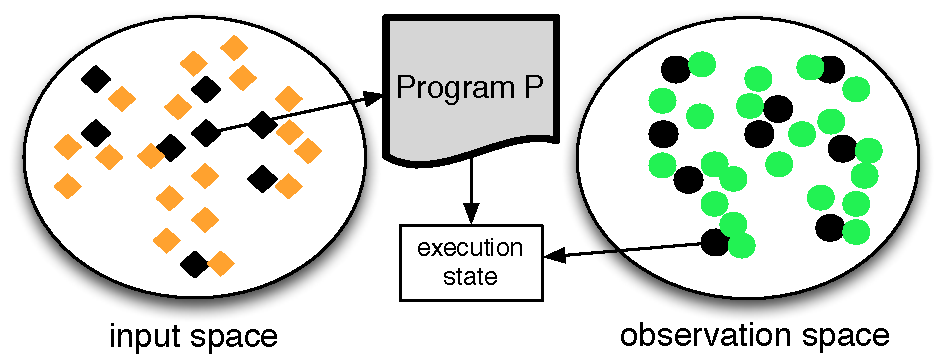
\includegraphics[scale=0.45]{io-spaces.pdf}

    % \fbox{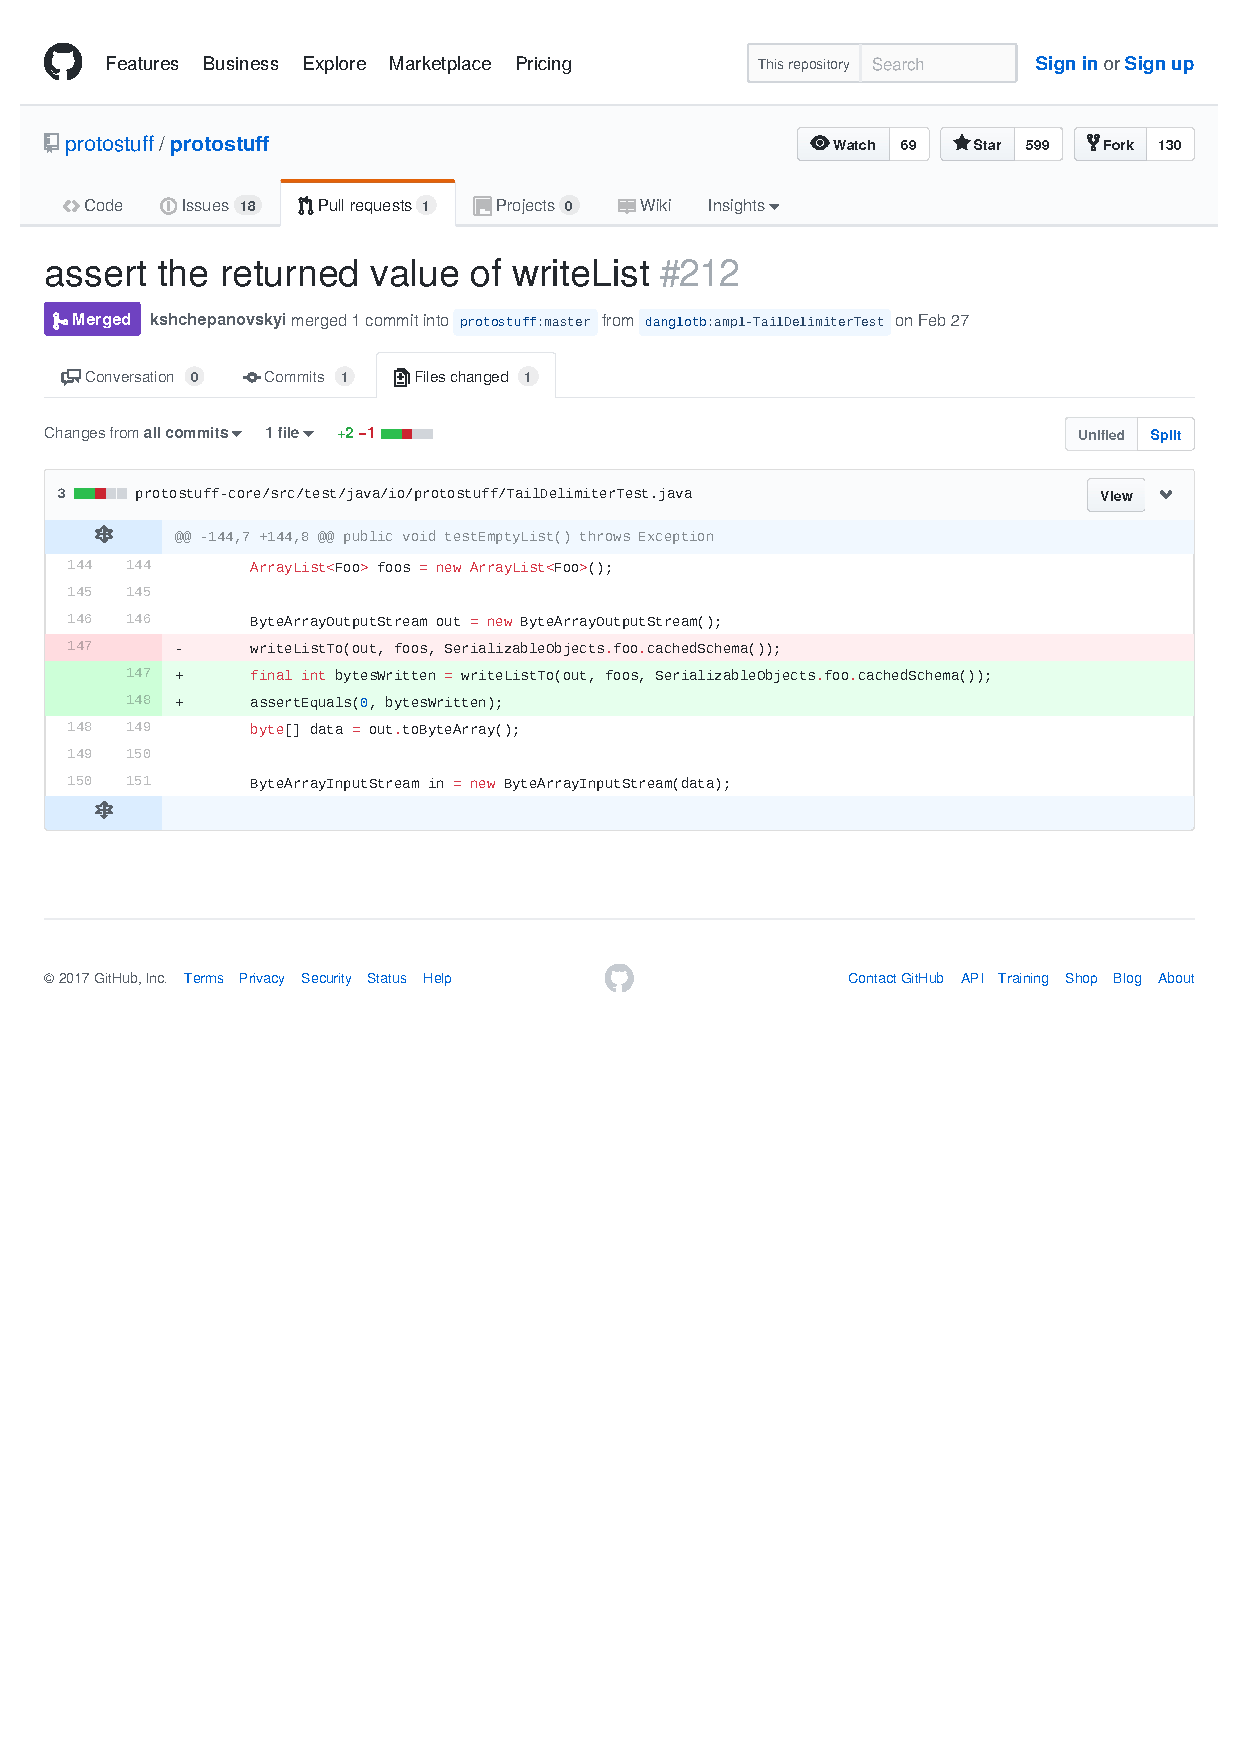
\includegraphics[trim=2cm 17.02cm 4.09cm 10.46cm, clip, width=\textwidth]{rq3_resources/protostuff.pdf}}
  \end{center}

  \pause{}

  \alert{New tests should be approved by the developers.}
\end{frame}
\begin{frame}{DSpot~\footcite{baudry2015dspot} --- Amplification Operators}
  \begin{description}
    \item[Literals] replaced with neighbor values.
    \item[Method calls] duplicated, removed or made-up (with random or default parameters).
  \end{description}
  Operators are not stacked.

  \vfill
  \pause{}

  \begin{description}
    \item[Assertions] generated to capture the state of the system after the test's execution.
  \end{description}
\end{frame}


\section{Planned Work}

\begin{frame}{Easing the Review Process}
  Developers have to review generated tests.
  \begin{itemize}
    \item Adding explanations: we have to make it easier for them to understand what the target of the new test is.
    \item Misunderstood tests are ignored or labelled as false-positive.
    \item Tests should be ordered as to present the most important ones first.
  \end{itemize}
\end{frame}

\begin{frame}{Efficient Generation}
  Generating a minimal set of tests would also reduce the work of developers \textbf{if} each test stays simple and logical.

  Stacking operators could allow the generation of tests covering more properties.
  \begin{itemize}
    \item Increases the search space, study the usefulness of each operator.
  \end{itemize}
\end{frame}


\section*{Conclusion}

\begin{frame}{Summary}
  \begin{enumerate}
    \item Practitioners need help designing good quality test suites.
    \item Automated techniques are available to enhance hand-written test.
    \item Search spaces are vast and tests need to be precise and follow a human-like logic.
    \item The internship will focus on adapting automated techniques for human interactions needs.
  \end{enumerate}
\end{frame}

\begin{frame}[standout]
  Thank you.
\end{frame}

\appendix

\end{document}
